%%%%%%%%%%%%%%%%%%%%%%%%%%%%%%%%%%%%%%%%%%%%%%%%%%%%%%%%%%%%%%%%%%%%%%%%%%%

\documentclass{standalone}

\usepackage{amsmath}
\usepackage{mathptmx}
\usepackage{tikz}
\usetikzlibrary{external}
\tikzexternalize{rectangular-fence}

%% IEEE uses Times Roman font, so we'll default to Times.
%% These three commands make up the entire times.sty package.
\renewcommand{\rmdefault}{ptm}
\renewcommand{\ttdefault}{pcr}
\normalfont\selectfont

%%%%%%%%%%%%%%%%%%%%%%%%%%%%%%%%%%%%%%%%%%%%%%%%%%%%%%%%%%%%%%%%%%%%%%%%%%%
%% A rectangular region.
%%%%%%%%%%%%%%%%%%%%%%%%%%%%%%%%%%%%%%%%%%%%%%%%%%%%%%%%%%%%%%%%%%%%%%%%%%%

\begin{document}

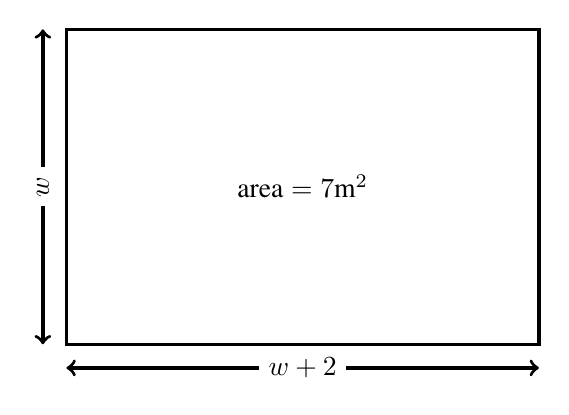
\begin{tikzpicture}[%%
  arrowStyle/.style={<->,very thick},%%
  labelStyle/.style={fill=white},%%
  lineStyle/.style={-,very thick}%%
]
%%
%%
\pgfmathsetmacro{\dx}{0.3}
\pgfmathsetmacro{\dy}{\dx}
\pgfmathsetmacro{\length}{6}
\pgfmathsetmacro{\width}{4}
\pgfmathsetmacro{\xlow}{0}
\pgfmathsetmacro{\ylow}{\xlow}
%%
\coordinate (lowerLeft) at (\xlow,\ylow);
\coordinate (upperRight) at (\length,\width);
%%
\normalsize
%% Draw the rectangular region and label its dimensions.
\draw[lineStyle] (lowerLeft) rectangle (upperRight);
%% Label the length.
\draw[arrowStyle] (\xlow,-\dy) -- (\length,-\dy);
\node[labelStyle] at (\length/2,-\dy) {$w + 2$};
%% Label the width.
\draw[arrowStyle] (-\dx,\ylow) -- (-\dx,\width);
\node[labelStyle,rotate=90] at (-\dx,\width/2) {$w$};
%% Label the area of the rectangular region.
\node[] at (\length/2,\width/2) {$\text{area} = 7\text{m}^2$};
\end{tikzpicture}

\end{document}
